\pagestyle{fancy}
\chapter{Θεωρία και Μεθοδολογία}
\section{Θεωρία}
Με δεδομένες τις διαστάσεις σε κάτοψη του στοιχείου θεμελίωσης, όπως αυτές αναφέρονται στον (Πίν. \ref{tab:geometry}), θεωρείται πως έχει προηγηθεί επιτυχώς ο έλεγχος της φέρουσας ικανότητας του εδάφους. Κριτήριο στο παρόν στάδιο είναι η αντοχή του ίδιου του πεδίλου.

Όλοι οι έλεγχοι αντοχής του πεδίλου γίνονται με υπόθεση γραμμικής κατανομής τάσεων εδάφους ${\sigma}$ κατά τις διευθύνσεις $x$ και $y$. Οι έλεγχοι αυτοί θεωρούν δηλαδή, ότι το πέδιλο μπορεί να αστοχήσει προτού το έδαφος φτάσει τη φέρουσα ικανότητά του. Επιπλέον, η επίπεδη κατανομή τάσεων οδηγεί, για την ίδια θέση της συνισταμένης δύναμης $N_{tot}$, σε μεγαλύτερες τάσεις εδάφους κοντά στην περίμετρο απ' ότι η υπόθεση σταθερών τάσεων εδάφους, άρα είναι δυσμενέστερη (ασφαλέστερη) για την αντοχή του ίδιου του πεδίλου.

\section{Μεθοδολογία}
Σε αυτό το σημείο ας ορίσουμε τρία μεγέθη που είναι απαραίτητα για τη συνέχεια. Οι ροπές $M_{x}$ και $M_{y}$ στο κέντρο της βάσης του πεδίλου ισοδυναμούν με δράση της $N_{tot}$ με εκκεντρότητες $e_{x}$ και $e_{y}$ κατά τους άξονες $x$ και $y$ αντίστοιχα.
\begin{equation}
  N_{tot} = N + A_f ({\gamma}_c h + {\gamma}_{\varepsilon\delta}(t_{\varepsilon\delta} - h)),\text{ όπου } A_f = b_x b_y
\end{equation}

\begin{subequations}
\begin{align}
  e_{x} & = \dfrac{M_{x}}{N_{tot}} \\[10pt]
  e_{y} & = \dfrac{M_{y}}{N_{tot}}
\end{align}
\end{subequations}

\subsection{Διάτμηση}
Ο έλεγχος σε διάτμηση ξεκινά από μία κάθετη διατομή στο οριζόντιο επίπεδο που ορίζει το πέδιλο, σε απόσταση $d$ από την παρειά σύνδεσης πεδίλου - κατακόρυφου στοιχείου. Στη γενική περίπτωση υπάρχουν τέσσερις τέτοιες διατομές (Σχ. \ref{fig:shear}), δύο κάθετες στον άξονα $x$ και δύο στον $y$. Με την παραδοχή μονοαξονικής εκκεντρότητας, ορίζονται οι αποστάσεις των δύο διατομών από τον άξονα $y$, $s_x$ και $s'_x$ και οι αποστάσεις των άλλων δύο διατομών από τον άξονα $x$, $s_y$ και $s'_y$. Από τις δύο κάθετες σε κάθε άξονα διατομές, η μία είναι κρίσιμη (μεγαλύτερη τιμή τέμνουσας), συνεπώς καταλήγουμε σε δύο τέμνουσες σχεδιασμού, μία για κάθε διεύθυνση.

\begin{figure}[H]
	\centering
	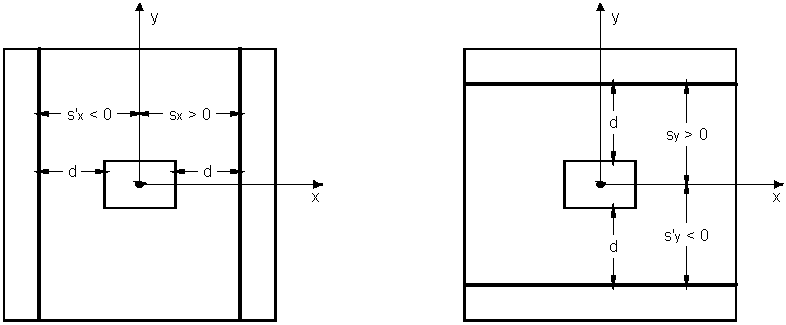
\includegraphics[scale=0.8]{shear}
	\caption{Κρίσιμες διατομές για τον έλεγχο πεδίλου σε διάτμηση}
	\label{fig:shear}
\end{figure}

Οι τέμνουσες σχεδιασμού σε κάθε μία από τις τέσσερις διατομές δίνονται από τις σχέσεις που ακολουθούν.

Για μονοαξονική εκκεντρότητα $e_{x}$ και $\dfrac{\abs{e_x}}{b_x} \leq \dfrac{1}{6}$:
\begin{subequations}
\begin{align}
  V_{Ed,x} & = N_{tot}\left(1 + \dfrac{3\abs{e_x}}{b_x}\left(1 + \dfrac{2s_x}{b_x}\right)\right)\left(0.5 - \dfrac{s_x}{b_x}\right) - \left(N_{tot} - N\right)\left(0.5 - \dfrac{s_x}{b_x}\right) \label{eqn:23a} \\[10pt]
  V'_{Ed,x} & = N_{tot}\left(1 - \dfrac{3\abs{e_x}}{b_x}\left(1 - \dfrac{2s'_x}{b_x}\right)\right)\left(0.5 + \dfrac{s'_x}{b_x}\right) - \left(N_{tot} - N\right)\left(0.5 + \dfrac{s'_x}{b_x}\right) \label{eqn:23b}
\end{align}
\end{subequations}

Για μονοαξονική εκκεντρότητα $e_{x}$ και $\dfrac{\abs{e_x}}{b_x} > \dfrac{1}{6}$:
\begin{subequations}
\begin{align}
  V_{Ed,x} & = \dfrac{4}{9}N_{tot}\dfrac{\left(2.5 - \dfrac{6\abs{e_x}}{b_x} + \dfrac{s_x}{b_x}\right)\left(0.5 - \dfrac{s_x}{b_x}\right)}{\left(1-\dfrac{2\abs{e_x}}{b_x}\right)^2} - \left(N_{tot} - N\right)\left(0.5 - \dfrac{s_x}{b_x}\right) \label{eqn:24a} \\[10pt]
  V'_{Ed,x} & = \dfrac{4}{9}N_{tot}\dfrac{\left(1 - \dfrac{3\abs{e_x}}{b_x} + \dfrac{s'_x}{b_x}\right)^2}{\left(1-\dfrac{2\abs{e_x}}{b_x}\right)^2} - \left(N_{tot} - N\right)\left(0.5 + \dfrac{s'_x}{b_x}\right) \label{eqn:24b}
\end{align}
\end{subequations}

Για μονοαξονική εκκεντρότητα $e_{y}$ και $\dfrac{\abs{e_y}}{b_y} \leq \dfrac{1}{6}$:
\begin{subequations}
\begin{align}
  V_{Ed,y} & = N_{tot}\left(1 + \dfrac{3\abs{e_y}}{b_y}\left(1 + \dfrac{2s_y}{b_y}\right)\right)\left(0.5 - \dfrac{s_y}{b_y}\right) - \left(N_{tot} - N\right)\left(0.5 - \dfrac{s_y}{b_y}\right) \label{eqn:25a} \\[10pt]
  V'_{Ed,y} & = N_{tot}\left(1 - \dfrac{3\abs{e_y}}{b_y}\left(1 - \dfrac{2s'_y}{b_y}\right)\right)\left(0.5 + \dfrac{s'_y}{b_y}\right) - \left(N_{tot} - N\right)\left(0.5 + \dfrac{s'_y}{b_y}\right) \label{eqn:25b}
\end{align}
\end{subequations}

Για μονοαξονική εκκεντρότητα $e_{y}$ και $\dfrac{\abs{e_y}}{b_y} > \dfrac{1}{6}$:
\begin{subequations}
\begin{align}
  V_{Ed,y} & = \dfrac{4}{9}N_{tot}\dfrac{\left(2.5 - \dfrac{6\abs{e_y}}{b_y} + \dfrac{s_y}{b_y}\right)\left(0.5 - \dfrac{s_y}{b_y}\right)}{\left(1-\dfrac{2\abs{e_y}}{b_y}\right)^2} - \left(N_{tot} - N\right)\left(0.5 - \dfrac{s_y}{b_y}\right) \label{eqn:26a} \\[10pt]
  V'_{Ed,y} & = \dfrac{4}{9}N_{tot}\dfrac{\left(1 - \dfrac{3\abs{e_y}}{b_y} + \dfrac{s'_y}{b_y}\right)^2}{\left(1-\dfrac{2\abs{e_y}}{b_y}\right)^2} - \left(N_{tot} - N\right)\left(0.5 + \dfrac{s'_y}{b_y}\right) \label{eqn:26b}
\end{align}
\end{subequations}

Οι δύο κρίσιμες τέμνουσες σχεδιασμού συγκρίνονται με την αντοχή σε τέμνουσα ανά διεύθυνση. Ελέγχεται δηλαδή αν:
\begin{subequations}
\begin{align}
  V_{Ed,x} \leq V_{Rd1,x} & = \left(\max\left\{\dfrac{180}{{\gamma}_c}\left(100{\rho}_{1,x}\right)^{1/3}, 35\sqrt{1 + \sqrt{\dfrac{0.2}{d}}}{f_{ck}}^{1/6}\right\}\left(1 + \sqrt{\dfrac{0.2}{d}}\right){f_{ck}}^{1/3}\right){b_y}d\label{eqn:27a}\\[10pt]
  V_{Ed,y} \leq V_{Rd1,y} & = \left(\max\left\{\dfrac{180}{{\gamma}_c}\left(100{\rho}_{1,y}\right)^{1/3}, 35\sqrt{1 + \sqrt{\dfrac{0.2}{d}}}{f_{ck}}^{1/6}\right\}\left(1 + \sqrt{\dfrac{0.2}{d}}\right){f_{ck}}^{1/3}\right){b_x}d\label{eqn:27b}
\end{align}
\end{subequations}

Όπου ${\gamma}_c = 1.5$ και ${\rho}_{1,x}$, ${\rho}_{1,y}$ τα γεωμετρικά ποσοστά των ράβδων οπλισμού της κάτω επιφάνειας που διαπερνούν τις κρίσιμες διατομές.

\subsection{Διάτρηση}
